%============================================================
			\section{Nombre: Salto de altura.} \label{hab.SalAl}
			\subsection{Descripción}
			El enemigo describe un desplazamiento convexo de gran velocidad. 
			\subsection{Portador}
			Jaguar. Ver \ref{per.jaguar}.
			\subsection{Esquema}
			Ver figura \ref{fig:SalAl}.
			\begin{figure}
				\centering
				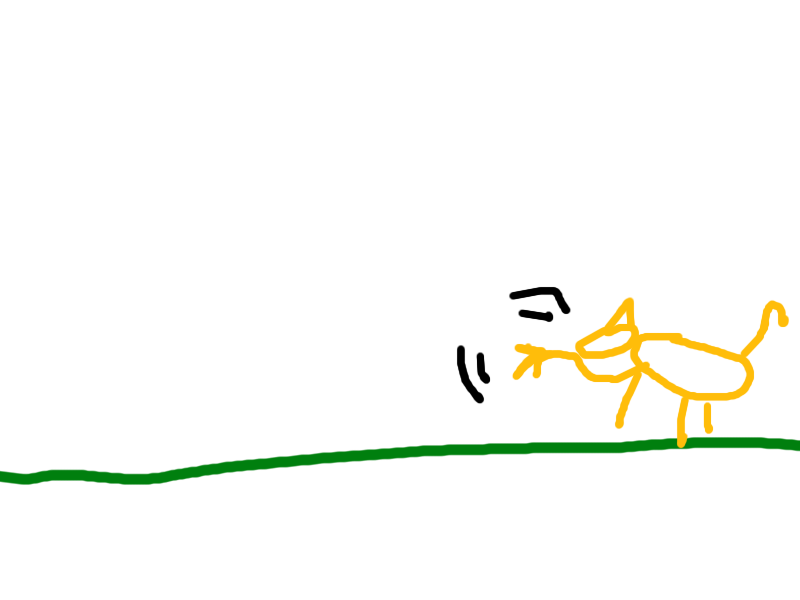
\includegraphics[height=0.2 \textheight]{Imagenes/zarpazo}
				\caption{Salto de altura.}
				\label{fig:SalAl}
			\end{figure}